\documentclass[10pt, a4paper]{report}
\usepackage[utf8]{inputenc}

\usepackage[T1]{fontenc}
\usepackage[english, french]{babel}
\usepackage{graphicx}
\usepackage{fullpage}
\usepackage{eso-pic}
\usepackage{tcolorbox}
\usepackage{hyperref}
\usepackage[toc]{glossaries}
\usepackage{tikz}

\usepackage{listings}
\usepackage{background}
\usepackage{setspace}
\usepackage{titlepic}

\usepackage{hyperref}
\usepackage{natbib}

% Définir les paramètres de l'image de fond pour la première page
\backgroundsetup{
	scale=2.5, % Échelle de l'image
	color=black, % Couleur de l'image (noir et blanc par défaut)
	opacity=0.1, % Opacité de l'image
	angle=0, % Angle de rotation de l'image
	position=current page.center, % Position de l'image centrée
	vshift=0cm, % Décalage vertical
	hshift=0cm, % Décalage horizontal
	contents={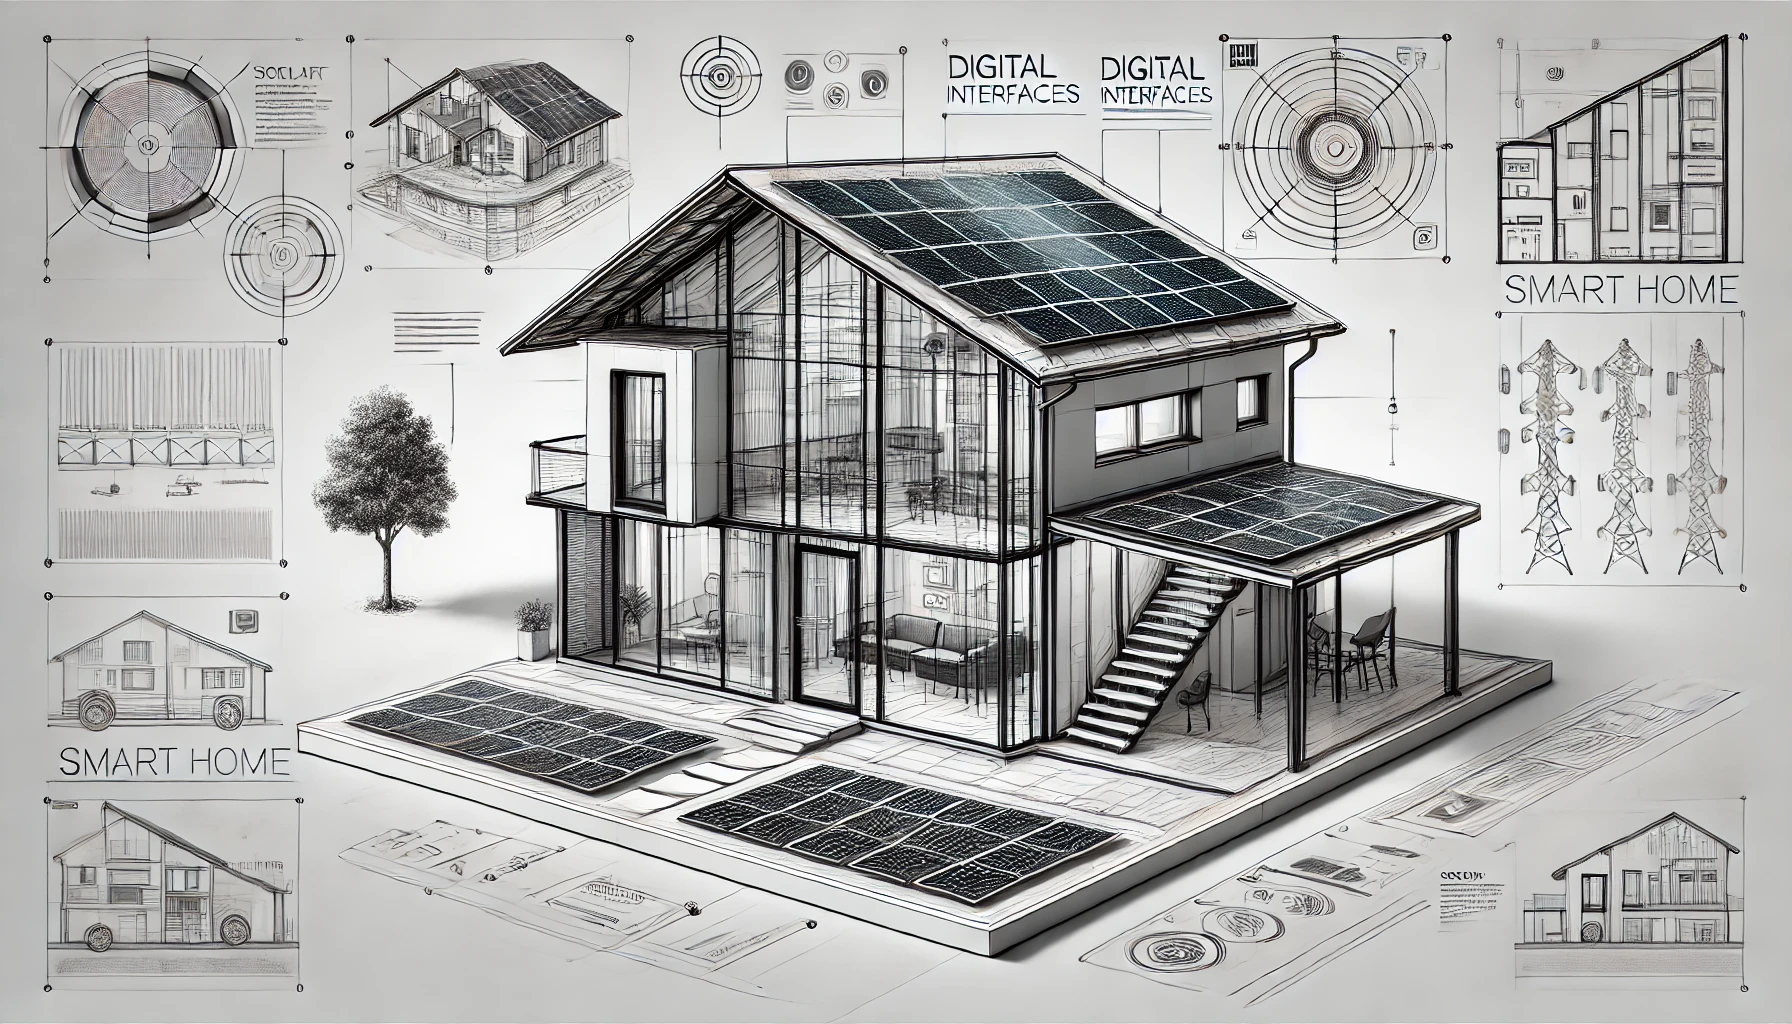
\includegraphics[width=\paperwidth]{ressources/img/logos/imageSmartHouse}} % Contenu (image de fond)
}

\usepackage[a4paper, top=2.5cm, bottom=2.5cm, left=3cm, right=2cm]{geometry}

% Pour la lisibilité, on peut utiliser le package setspace pour ajuster l'espacement entre les lignes
\usepackage{setspace}
\usetikzlibrary{positioning, decorations.pathreplacing}

\definecolor{darkWhite}{rgb}{0.94,0.94,0.94}

\lstset{
	aboveskip=3mm,
	belowskip=-2mm,
	backgroundcolor=\color{darkWhite},
	basicstyle=\footnotesize,
	breakatwhitespace=false,
	breaklines=true,
	captionpos=b,
	commentstyle=\color{red},
	deletekeywords={...},
	escapeinside={\%*}{*)},
	extendedchars=true,
	framexleftmargin=16pt,
	framextopmargin=3pt,
	framexbottommargin=6pt,
	frame=tb,
	keepspaces=true,
	keywordstyle=\color{blue},
	language=Python,
	literate=
	{²}{{\textsuperscript{2}}}1
	{⁴}{{\textsuperscript{4}}}1
	{⁶}{{\textsuperscript{6}}}1
	{⁸}{{\textsuperscript{8}}}1
	{€}{{\euro{}}}1
	{é}{{\'e}}1
	{è}{{\`{e}}}1
	{ê}{{\^{e}}}1
	{ë}{{\¨{e}}}1
	{É}{{\'{E}}}1
	{Ê}{{\^{E}}}1
	{û}{{\^{u}}}1
	{ù}{{\`{u}}}1
	{â}{{\^{a}}}1
	{à}{{\`{a}}}1
	{á}{{\'{a}}}1
	{ã}{{\~{a}}}1
	{Á}{{\'{A}}}1
	{Â}{{\^{A}}}1
	{Ã}{{\~{A}}}1
	{ç}{{\c{c}}}1
	{Ç}{{\c{C}}}1
	{õ}{{\~{o}}}1
	{ó}{{\'{o}}}1
	{ô}{{\^{o}}}1
	{Õ}{{\~{O}}}1
	{Ó}{{\'{O}}}1
	{Ô}{{\^{O}}}1
	{î}{{\^{i}}}1
	{Î}{{\^{I}}}1
	{í}{{\'{i}}}1
	{Í}{{\~{Í}}}1,
	morekeywords={*,...},
	numbers=left,
	numbersep=10pt,
	numberstyle=\tiny\color{black},
	rulecolor=\color{black},
	showspaces=false,
	showstringspaces=false,
	showtabs=false,
	stepnumber=1,
	stringstyle=\color{gray},
	tabsize=4,
	title=\lstname,
}

% Additional language definitions
\lstdefinelanguage{JavaScript}{
	keywords={typeof, new, true, false, catch, function, return, null, catch, switch, var, if, in, while, do, else, case, break},
	keywordstyle=\color{blue}\bfseries,
	ndkeywords={class, export, boolean, throw, implements, import, this},
	ndkeywordstyle=\color{darkgray}\bfseries,
	identifierstyle=\color{black},
	sensitive=false,
	comment=[l]{//},
	morecomment=[s]{/*}{*/},
	commentstyle=\color{purple}\ttfamily,
	stringstyle=\color{orange}\ttfamily,
	morestring=[b]',
	morestring=[b]"
}

\lstdefinelanguage{C}{
	keywords={auto, break, case, const, continue, default, do, double, else, enum, extern, float, for, goto, if, inline, int, long, register, restrict, return, short, signed, sizeof, static, struct, switch, typedef, union, unsigned, void, volatile, while, _Bool, _Complex, _Imaginary},
	keywordstyle=\color{blue}\bfseries,
	identifierstyle=\color{black},
	sensitive=true,
	comment=[l]{//},
	morecomment=[s]{/*}{*/},
	commentstyle=\color{green}\ttfamily,
	stringstyle=\color{red}\ttfamily,
	morestring=[b]',
	morestring=[b]"
}

\makeglossaries
\newglossaryentry{API}
{
	name=API,
	description={(Interface de Programmation d'Application) est un ensemble de protocole permettant à différentes applications logicielle d'echanger des données entre elles}
}

\newcommand{\HRule}{\rule{\linewidth}{0.5mm}}
\newcommand{\blap}[1]{\vbox to 0pt{#1\vss}}
\newcommand\AtUpperLeftCorner[3]{%
	\put(\LenToUnit{#1},\LenToUnit{\dimexpr\paperheight-#2}){\blap{#3}}%
}
\newcommand\AtUpperRightCorner[3]{%
	\put(\LenToUnit{\dimexpr\paperwidth-#1},\LenToUnit{\dimexpr\paperheight-#2}){\blap{\llap{#3}}}%
}

\title{\LARGE{Smarthouse}}
\author{\textsc{Khedhaouria} Eliès \& \textsc{Marcelet} Paul}
\date{\today}
\makeatletter



\begin{document}
	\onehalfspacing % Définit l'espacement entre les lignes à 1.5
	
	
	\begin{titlepage}
		
		
		\enlargethispage{2cm}
		
		\AddToShipoutPicture{
			\AtUpperLeftCorner{1.5cm}{1cm}{
\includegraphics[width=6.5cm]{ressources/img/logos/isimaInp.png}}
		}
		
		\begin{center}
			\vspace*{10cm}
			
			\LARGE{\textbf{Rapport d'élève Ingénieur}}\\
			\LARGE{\textbf{Projet de troisième année}}\\
			\large{Filière:\textbf{ Sécurité} et \textbf{réseaux}} 
			\HRule
			\vspace*{0.5cm}
			\Huge{\textsc{\textbf{\@title}}}\\
			
		\end{center}
		\vspace*{2.5cm}
		Présenté par: \textbf{\@author }
		
		\vspace*{4.5cm}
		Responsable Isima: Monsieur \textbf{Alexandre GUITTON} \hspace*{2cm} Date de soutenance: \textbf{02/07/2024}\\\\
		\textbf{Campus des Cézeaux .  1 rue de la Chébarde .  TSA 60125 .  63178  Aubière CEDEX}
		
		
		
	\end{titlepage}
	\backgroundsetup{contents={}}
	\ClearShipoutPicture
	\newpage
	
	\section*{Remerciements}
	
	\tableofcontents
	\listoffigures
	
	\begin{abstract}
		\selectlanguage{french}
	Dans le cadre de notre \textbf{projet de fin d’études}, nous avons conçu et développé un \textbf{système de maison intelligente} 
	capable de transmettre \textbf{des données en temps réel de manière sécurisée} vers un serveur distant. L’objectif principal est de 
	mettre en place un \textbf{système de monitoring avancé}, permettant à un propriétaire de superviser et d’analyser les données 
	générées par ses équipements connectés.
	
	Pour garantir \textbf{l’intégrité et la confidentialité des échanges}, nous avons implémenté une \textbf{communication sécurisée 
	basée sur des certificats SSL/TLS} et le protocole \textbf{MQTTs}, assurant ainsi une transmission chiffrée et authentifiée entre 
	la maison et le serveur.
	
	Les données collectées par les capteurs sont stockées dans une \textbf{base de données à série temporelle} (InfluxDB), 
	spécialement optimisée pour le traitement et l’analyse de données en flux continu.
	
	Une \textbf{API centralisée}, développée en \textbf{Laravel}, a été mise en place afin de :
	\begin{itemize}
		\item \textbf{Gérer la création des propriétaires} et l’association sécurisée de leurs équipements.
		\item \textbf{Automatiser la génération et la signature des certificats} pour garantir une authentification fiable.
		\item \textbf{Offrir une interface d’accès aux données}, permettant aux utilisateurs de récupérer \textbf{des données en temps 
		réel ou historiques}, selon différents filtres appliqués à la base de données.
	\end{itemize}
	
	Enfin, une \textbf{interface graphique interactive}, développée en \textbf{Qt}, permet aux utilisateurs de \textbf{visualiser les 
	données en temps réel} sous forme de \textbf{graphiques dynamiques}. Cette interface interagit directement avec l’API afin de 
	récupérer et d’afficher \textbf{les données filtrées}, qu’elles soient en temps réel ou issues d’une période spécifique dans le 
	passé.
	
	Ce projet intègre \textbf{des technologies modernes et des concepts avancés en sécurité, IoT, gestion des bases de données et 
	visualisation de données en temps réel}, assurant ainsi une \textbf{infrastructure robuste, fiable et évolutive}.

	\end{abstract}
	\selectlanguage{english}
	\begin{abstract}
		As part of our \textbf{final-year engineering project}, we designed and developed a \textbf{smart home system} capable of 
		securely transmitting \textbf{real-time data} to a remote server. The main objective is to implement an \textbf{advanced 
		monitoring system} that allows a homeowner to monitor and analyze data generated by their connected devices.
		
		To ensure \textbf{data integrity and confidentiality}, we implemented a \textbf{secure communication protocol based on SSL/TLS 
		certificates} and the \textbf{MQTTs protocol}, providing encrypted and authenticated communication between the home and the 
		server.
		
		Sensor data is stored in a \textbf{time-series database} (InfluxDB), optimized for real-time data processing and analysis.
		
		A \textbf{centralized API}, developed in \textbf{Laravel}, has been implemented to:
		\begin{itemize}
			\item \textbf{Manage the creation of homeowners} and the secure association of their devices.
			\item \textbf{Automate the generation and signing of certificates} to ensure reliable authentication.
			\item \textbf{Provide a data access interface}, allowing users to retrieve \textbf{real-time or historical data} based on 
			various filters applied to the database.
		\end{itemize}
		
		Finally, an \textbf{interactive graphical interface}, developed in \textbf{Qt}, allows users to \textbf{visualize real-time 
		data} using \textbf{dynamic graphs}. This interface directly interacts with the API to retrieve and display \textbf{filtered 
		data}, whether in real-time or from a specific historical period.
		
		This project integrates \textbf{modern technologies and advanced concepts in security, IoT, database management, and real-time 
		data visualization}, ensuring a \textbf{robust, reliable, and scalable infrastructure}.
		
	\end{abstract}
	
	
	\chapter{Introduction}
		La \textbf{domotique} représente aujourd'hui un enjeu majeur dans le domaine des innovations technologiques. Avec l'essor des 
		\textbf{maisons connectées} et des \textbf{IOTs}, les utilisateurs peuvent désormais \textbf{surveiller} et \textbf{contrôler} 
		leur domicile à distance, leur assurant ainsi une amélioration significative en termes de \textbf{sécurité}, 
		\textbf{d'efficacité énérgétique} et de \textbf{confort}. Cette évolution s'inscrit dans un contexte plus large dans lequel 
		l'automatisation et la connectivité jouent un rôle crucial dans notre quotidien.\\
		Le \textbf{monitoring à distance} des équipements d'une maison constitue un axe fondamental de la domotique moderne. Il permet 
		aux propriétaires d'obtenir une \textbf{vue globale de l'état de leur habitation en temps réel}. Cela joue un rôle crucial dans 
		plusieurs domaines:\\
		\begin{itemize}
			\item Il permet de \textbf{sécuriser} un domicile, permettant par exemple la détéction d'intrusion ainsi que la prévention 
			des cambriolages
			
			\item Il permet également une \textbf{optimisation énérgétique} du domicile, par le biais de l'automatisation des objets 
			connectés, en fonction d'horraires programmés, afin d'optimiser la consommation d'énergie.
			
			\item Il permet enfin \textbf{un confort et un contrôle à distance}, offrant aux propriétaires la possibilité d'activer ou 
			de désactiver certains dispositifs sans être physiquement présent.
		\end{itemize}
		Si ces avancées technologiques offrent des opportunités considérables, elles soulèvent néanmoins une problématique critique: 
		\textbf{la sécurisation des dispositifs IoTs et du transfert des données}. Aujourd'hui, de nombreux objets connectés sont 
		déployés avec des failles de sécurité importantes souvent négligées par les fabricants et les utilisateurs. Des outils comme 
		\textbf{Shodan}, un moteur de recherche spécialisé dans l'identification des appareils connectés exposés sur Internet, mettent 
		en évidence la vulnérabilité de nombreux systèmes IoTs accessibles sans protection adéquate. Cette situation constitue un risque 
		majeur, rendant possible des cyberattaques capables de compromettre \textbf{l'intégrité} et \textbf{la confidentialité} des 
		données échangées.\\
		Ce rapport décrit une architecture, solution à cette problématique en explorant l'une des applications majeures de la domotique: 
		\textbf{le monitoring à distance des capteurs d'une maison connectée, ainsi que l'établissement d'une communication sécurisée et 
		authentifiée entre celle-ci et un serveur distant}. L'objectif est de permettre aux utilisateurs de récupérer des \textbf{données 
		en temps réel}, issues de capteurs de leur domicile tout en garantissant \textbf{une transmission chiffrée} afin de protéger les 
		échanges contre d'éventuelles interceptions malveillantes. C'est à partir de cela que l'on peut définir une problématique à 
		laquelle la solution doit répondre: \textbf{Comment développer un système de monitoring en temps réel pour une maison connectée, 
		garantissant la sécurité de la transmission des données tout en renforcant l'authentification des équipements IoTs ?}
		
	
	\chapter{Contexte du Projet}
	\section{Analyse du besoin et définition des objectifs}
	\section{Organisation de la conception à la création}
	
	\chapter{État de l'Art}
	\section{Technologies existantes}
	\section{Solutions alternatives et justification des choix}
	
	\chapter{Conception et Implémentation}
	
	\section{Infrastructure et Environnement de Développement}
	
	\subsection{Simulation du serveur et architecture réseau}
	\subsubsection{Déploiement d'un Broker MQTT sécurisé}
	\subsubsection{Intégration d'une base de données à séries temporelles}
	\subsubsection{Formalisation des données entre Mosquitto et InfluxDB}
	
	\subsection{Modélisation et Simulation d'une Maison Connectée}
	\subsubsection{Conception de l'architecture logicielle de la simulation}
	\subsubsection{Implémentation du protocole MQTTs}
	\subsubsection{Structuration et formalisation des données échangées}
	
	\section{Mise en place d'une API Web}
	\subsection{Architecture logicielle de l'API et choix technologiques}
	\subsection{Automatisation de l'authentification des maisons}
	\subsubsection{Mise en place d'une base de données MySQL}
	\subsubsection{Signature automatique des certificats}
	\subsection{Filtrage et récupération des données}
	\subsubsection{Communication avec InfluxDB API}
	
	\section{Surveillance des données avec une interface graphique}
	\subsection{Architecture logicielle de l'application SmartHouse Monitoring}
	\subsection{Intégration et communication avec l'API Web}
	\subsubsection{Authentification des maisons}
	\subsubsection{Affichage des données récupérées}
	
	\chapter{Résultats et Discussion}
	\section{Situation à la fin de l’étude}
	\section{Analyse des résultats obtenus}
	
	\chapter{Conclusion}
	\section{Conclusion du projet}
	\section{Limites et améliorations possibles}
	
	\appendix
	\chapter{Annexes}
	\section{Lexique}
	\section{Bibliographie}
	\section{Webographie}
	
	
	
		
	
	\nocite{*}
	\bibliographystyle{unsrt}
	\bibliography{references}
	
	\clearpage
	
	\printglossaries
	
	
\end{document}